\section{Kreuzvalidierung und Effizienz des k-NN-Klassifikators}

\subsection{Allgemeine Fragen zur Evaluation eines Klassifikators}

\subsubsection{Klassifikationsfehlerwahrscheinlichkeiten}
Die Klassifikationsfehlerwahrscheinlichkeit ist 0, da es nur einen nächsten Nachbarn gibt und somit nur eine Klasse, die zugewiesen wird. 


\subsubsection{Diskussion des Ergebnis der Klassifikationsfehlerwahrscheinlichkeit}
Ja, da diese auch immer nur einen Nachbar haben und somit nur einr Klasse zugeordnet werden können.

\subsubsection{Möglichkeiten, um einen realistischen Schätzwert des Generalisierungsfehlers zu erhalten}
Man kann für k einen größeren Wert wählen. 
\subsubsection{Begriff Kreuzvalidierung}
Die Daten werden in S Teile aufgeteilt von denen immer ein Teil zur Validierung zurückgehalten wird. Dabei wird das Modell S mal trainiert. Am Ende erhält man dadurch den resultierenden Generalisierungsfehler.

\subsection{Code-Review der Methode \textit{Classifier.crossvalidate(self, S, X, T)}}

\noindent
\textbf{Was bedeutet der Parameter S?}

\vspace{5px}
\noindent
Die Daten werden in S Daten aufgeteilt. Es wird immer ein Teil zum validieren zurückgehalten. 

\vspace{5px}
\noindent
\textbf{Welche Rolle spielen die Variablen perm sowie Xp und Tp?}

\vspace{5px}
\noindent
\textit{perm}: eine zufällige Permutation der Zahlen 0 bis N-1 wird in einem np.array abgelegt. Liefert zufällige Indizes für Xp und Tp.
\textit{Xp und Tp}: Daten aus X werden in zufälliger Reihenfolge in Xp abgelegt. Daten aus T werden in zufälliger Reihenfolge n Tp abgelegt.

\vspace{5px}
\noindent
\textbf{Welche Rolle spielt idxS?}

\vspace{5px}
\noindent
Was bewirkt die äußere Schleife for idxTest in idxS?
Durchläuft alle möglichen Datasets und holt sich die Indizes für Trainingsdaten und speichert diese in \textit{X\textunderscore learn} und \textit{T\textunderscore learn}. Die restlichen Daten sind Testdaten und werden in \textit{X\textunderscore test} und \textit{T\textunderscore test} gespeichert. 

\vspace{5px}
\noindent
\textbf{Was passiert für S=1?}

\vspace{5px}
\noindent
Für S=1 wird das gesamte Dataset zum Lernen und Trainieren verwendet.

\vspace{5px}
\noindent
\textbf{Was bewirkt die innere Schleife for i in range(len(X\textunderscore test)): …?}

\vspace{5px}
\noindent
Durchläuft alle Datenvektoren in \textit{X\textunderscore test} und klassifiziert diese, holt sich aus \textit{T\textunderscore test} das zugehörige „richtige“ Label und schreibt in die Matrix nC die Häufigkeit, wie oft das jeweilige Label aufkommt. Später wird die Anzahl der Fehler ausgewertet. 

\vspace{5px}
\noindent
\textbf{Was bedeuten die Ergebnisse der Kreuzvalidierung pClassError und pConfErrors?}

\vspace{5px}
\noindent
In pClassError wird aufsummiert, wie oft die Testdaten nicht korrekt klassifiziert wurden. Die Anzahl wird dann noch durch die Gesamtheit aller Datenvektoren geteilt, um die Wahrscheinlichkeit eines Klassifikationsfehlers zu erhalten.
In der Matrix pConfErrors ist auf der Hauptdiagonalen die Anzahl der Fälle, in denen die Testdaten korrekt klassifiziert wurden. Alle anderen Elemente der Matrix enthalten die Anzahl der Fälle, in denen die Testdaten nicht korrekt klassifiziert wurden. Alle Elemente der Matrix werden dann noch durch die Wahrscheinlichkeit für das Auftreten der jeweiligen Klasse geteilt. So erhält man die Wahrheitsmatrix. 

\subsection{Betrachtung eines 2-Klassen-Problems für Gauß-verteilte Datenvektoren $x_n \in \mathbb{R}^D$ mit D-dim. Dichtefunktion}

\vspace{5px}
\noindent
\textbf{Wozu benötigt man den Befehl \textit{from V1A2\textunderscore Classifier import $\ast$ }?}

\vspace{5px}
\noindent
Um die Funktionen die in \textit{V1A2\textunderscore Classifier.py} definiert und implementiert wurden, in \textit{V1A3\textunderscore CrossVal\textunderscore KNN.py} nutzen zu können. 

\vspace{5px}
\noindent
\textbf{Mit welchem Befehl werden die Gauß-verteilten Datenvektoren erzeugt?
Wie viele Datenpunkte werden generiert? Was bedeuten die Variablen N, N1, N2?}

\vspace{5px}
\noindent
Mit dem Befehl
\textit{$numpy.random.multivariate_normal(mean, cov[, size, check_valid, tol])$}
N1 und N2: Anzahl der Datenvektoren für die zwei Klassen. 
N: Anzahl der Datenvektoren von X1 und X2 insgesamt, also 1000.

\vspace{5px}
\noindent
\textbf{Welche klassenspezifischen Verteilungen haben die Daten?}

\vspace{5px}
\noindent
Klasse 1 Mittelwert: [1,1]
Klasse 2 Mittelwert: [3,1]
Klasse 1 Kovarianzmatrix: [ [1,0.5] [0.5,1] ]
Klasse 2 Kovarianzmatrix: [ [1,0.5] [0.5,1] ]

\vspace{5px}
\noindent
\textbf{Welche Bedeutung haben die Variablen pE\textunderscore naive,
pCE\textunderscore naive und t\textunderscore naive?}

\vspace{5px}
\noindent
pE\textunderscore naive: Wahrscheinlichkeit eines Klassifikationsfehlers\\
pCE\textunderscore naive: Wahrheitsmatrix\\
t\textunderscore naive: Berechnungszeit\\

 
\begin{figure}[H]
    \centering
    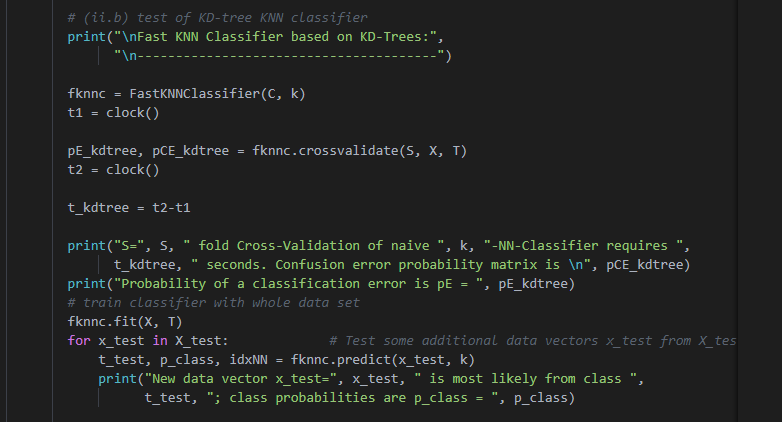
\includegraphics[width=1\linewidth]{files/aufgabe3c5.png}
    \caption{Codevervollständigung}
\end{figure}

\subsection{Test der Kreuzvalidierung bzw. Klassifikationsleistung}

\subsubsection{Bestimmung der Klassifikationsfehler und Verwechselwahrscheinlichkeiten}

\begin{figure}[H]
    \centering
    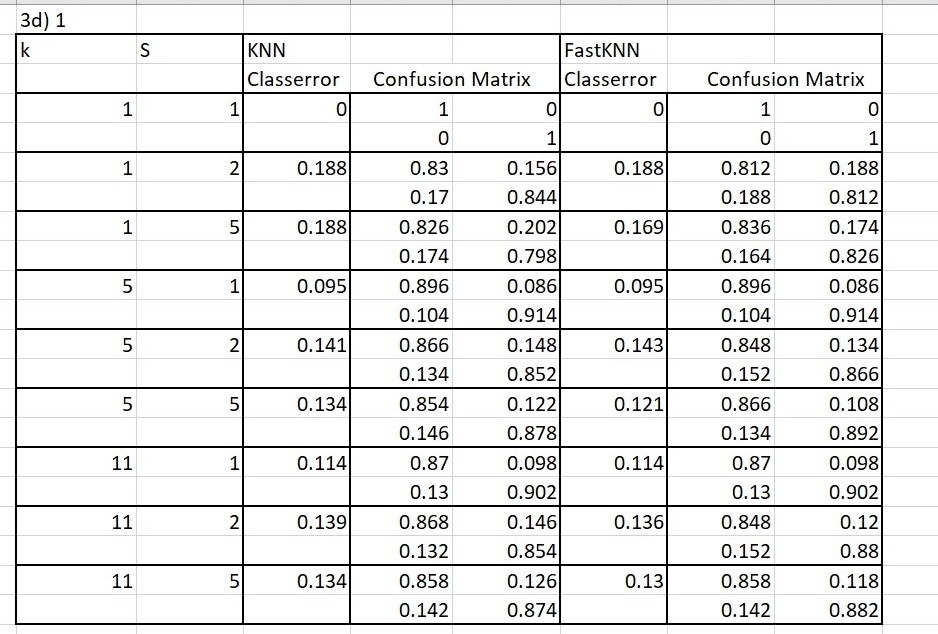
\includegraphics[width=1\linewidth]{files/aufgabe3d1.jpg}
    \caption{Wahrheitsmatrix}
\end{figure}

\subsubsection{Bestimmung der Klassenverteilung für drei weitere Testpunkte}

\begin{figure}[H]
    \centering
    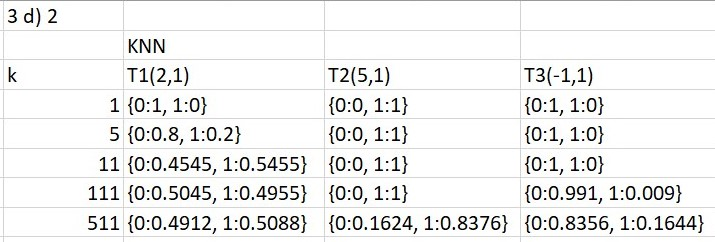
\includegraphics[width=1\linewidth]{files/aufgabe3d2.jpg}
    \caption{Klassenwahrscheinlichkeiten}
\end{figure}

\subsection{Vergleich der Effizienz beider k-NN-Klassifikatoren}


\begin{figure}[H]
    \centering
    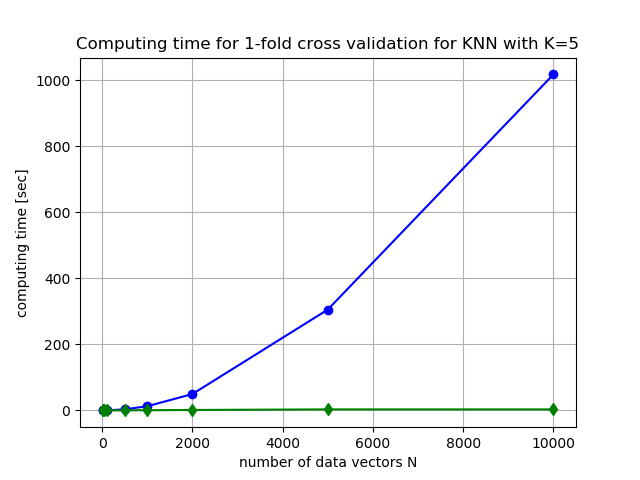
\includegraphics[width=1\linewidth]{files/laufzeitknn.png}
\end{figure}


\begin{figure}[H]
    \centering
    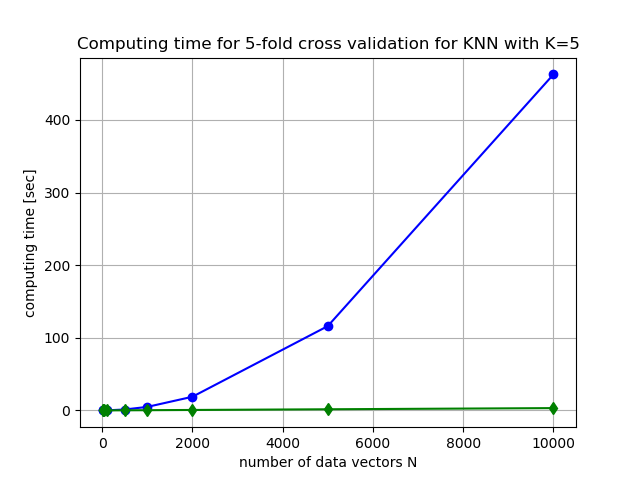
\includegraphics[width=1\linewidth]{files/laufzeitknn2.png}
\end{figure}